\section{Implementierung}
Dieses Kapitel beschreibt die Umsetzung des Projekts im Detail. Es wird ein Überblick über den Implementierungsprozesse gegeben, der Vorgehensweise bei der Entwicklung und ein Einblick in Probleme, welche während der Entwicklung aufgetreten sind.
Neben einer schrittweisen Darstellung der Implementierung werden auch exemplarisch Codebeispiele vorgestellt.
\subsection[Implementierungsdetails]{Implementierungsdetails}
In den Implementierungsdetails werden die Vorgehensweisen und Konzepte, welche für die Implementierung des Fontends und Backends benötigt werden, erläutert.

\subsubsection[Frontend]{Frontend}
Das \gls{sapui5}-Framework verwendet zur Darstellung der Seiten sogenannte \textit{Views} welche in \gls{xml} Dateien definiert werden.
Diese Views müssen mit der Dateiendung "\textbf{.view.xml}"\ enden, damit sie von \gls{sapui5} als View erkannt werden.

Views sind eine Art Container für \gls{sapui5}-Elemente (Buttons, Input Felder, Enitäten, Listen, ...) und \gls{sapui5}-Layouts (Flex Box, HBox, VBox).
Views können jedoch auch andere Views beinhalten und so einen verschachtelten Aufbau der Seite schaffen.
Die \gls{sapui5}-Elemente sind vorgefertigte Komponenten welche von \gls{sapui5} bereitgestellt werden, um eine einheitliche Benutzeroberfläche zu schaffen, welche dann auch über verschiedene SAP-Anwendungen in einem Unternehmen konsistent ist.

Für die Admin-UI Seite sollen die Views und Komponenten wie in Abbildung \ref{fig:appstructure} angeortnent und strukturiert werden.
Die Unterseiten für die Eingabefelder aus den Anforderungen \ref{Tab:A4}, \ref{Tab:A5} und \ref{Tab:A6} werden in eigenen Views angezeigt, zwischen denen der Benutzer über die Navigationsleiste wechseln kann.

\begin{figure}[H]
    \centering
    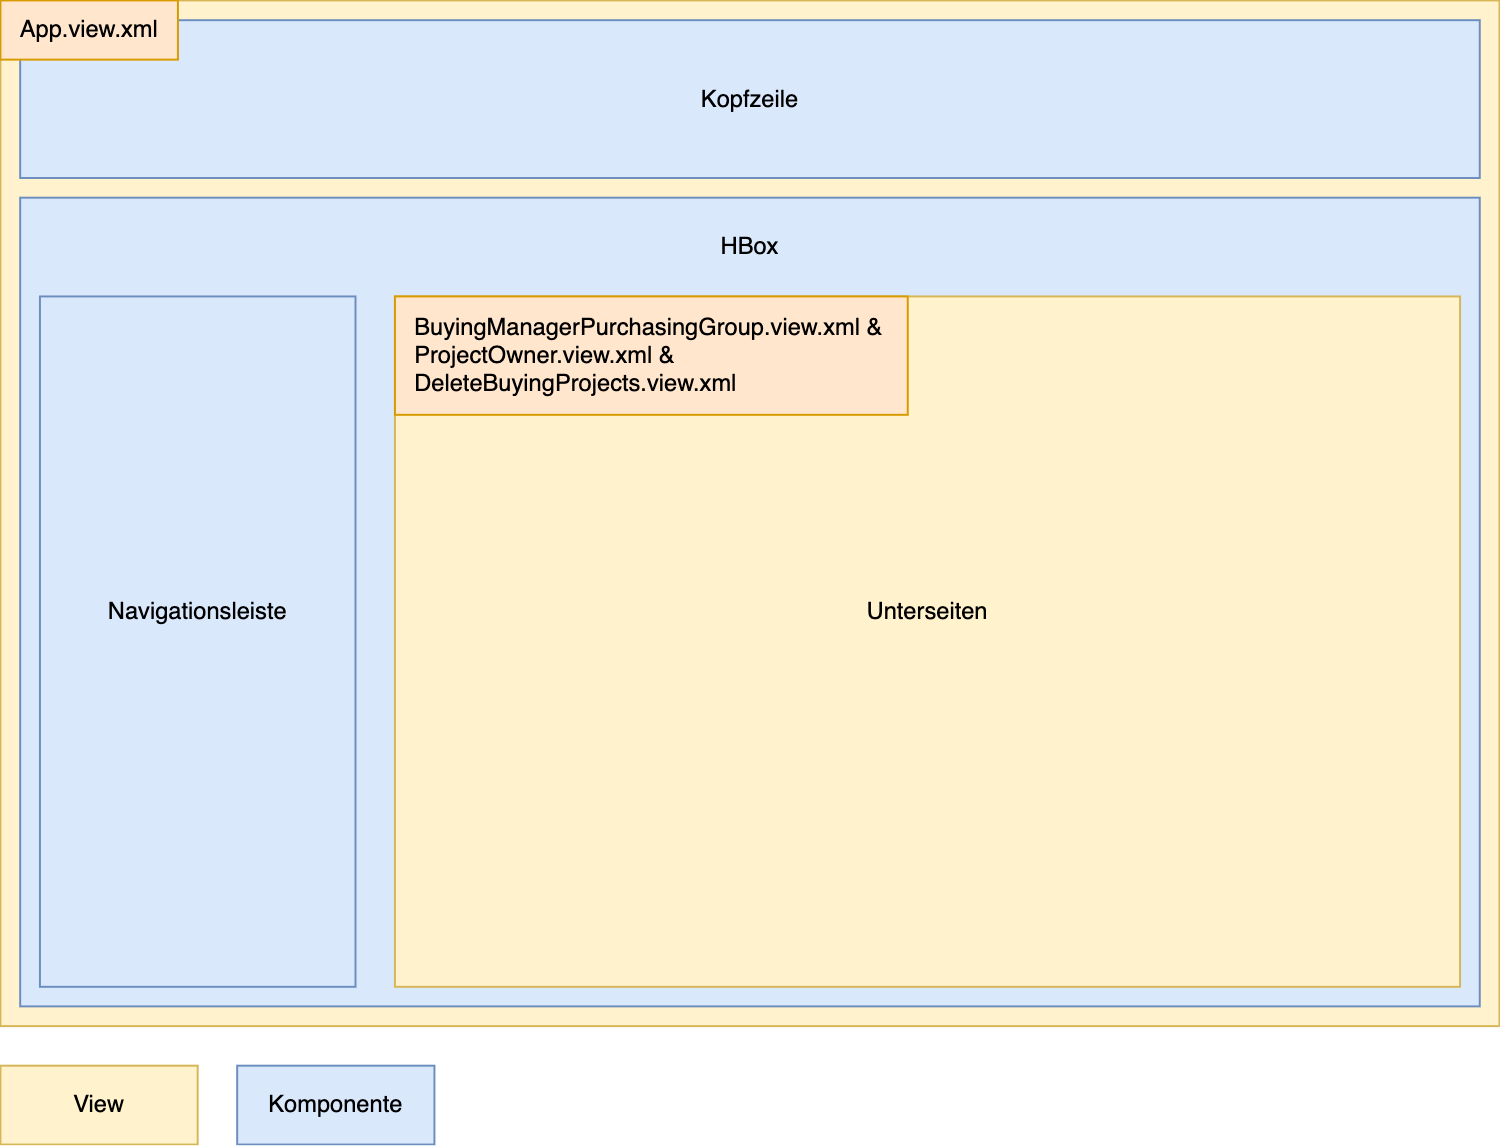
\includegraphics[width=\linewidth]{Images/AppStructure.png}
    \caption[Darstellung der Anwendungsstruktur]{Darstellung der Anwendungsstruktur}
    \label{fig:appstructure}
\end{figure}

Für jeden View kann ein \textit{Controller} erstellt werden, welcher die Funktionalität für die Views bereitstellt und Elemente dynamisch laden kann. 
Ein Controller muss, so wie die View, eine besondere Dateiendung haben, damit \gls{sapui5} die Datei als Controller erkennen kann. Für Controller ist diese Endung "\textbf{.controller.ts}".

Für das Admin-UI soll für jeden View ein Controller erstellt werden. Zudem soll es einen sogenannten \textit{BaseContoller} geben, von dem alle anderen Controller seine Funktionen erben.
Dieser BaseController benötigt, anders also normale Controller, nicht die Controller spezifische Endung, sondern nur die TypeScript-spezifische Dateiendung "\textbf{.ts}".
Denn der BaseController wird keinem View explizit zugeordnet und muss daher auch nicht von \gls{sapui5} als Controller erkannt werden.  

Die Funktion eines BaseControllers ist es, Funktionen, welche von jedem Controller benötigt werden, in diesem zu definieren, damit diese an einer zentralen Stelle definiert sind und nicht in jedem Controller neu defniert werden müssen. 
Dazu gehören meist Helferfunktionen für zum Beispiel das Routing oder im Fall des Admin-UIs auch die Funktionalität der Aktionsleiste (siehe Anforderung \ref{Tab:A7}), welche auf jeder Unterseite eine sehr ähnliche Funktion hat.

In den Controllern für die einzelnen Unterseiten sollen Funktionen, die spezifisch für die Unterseiten sind stehen, wie die intelligenten Vorschläge für die Eingabefelder (Anforderung \ref{Tab:A3}) und das Senden der Daten an das Backend.

\subsubsection[Backend]{Backend}
Im Backend sollen die Daten, welche von dem Frontend gesendet wurden, validiert und verarbeitet werden.

Für das Löschen eines Kaufprojekts muss lediglich die \textit{projectId} des zu löschenden Projektes gesendet werden, wofür eine \gls{cap} \textit{function} verwendet werden soll.

Für das Ändern der Projekt Owner und Manager, sowie der Purchasing Organisation, soll für jede Änderung ein neuer Eintrag in eine Datenbanktabelle geschrieben werden, der die alten und neuen Werte, sowie den Benutzer der die Änderung getätigt hat und den Zeitpunkt der Änderung beinhaltet.
Diese Datenbanktabellen sind in Abbildung \ref{fig:masschangetables} dargestellt.
Dies soll dazu dienen, die Änderungen auch im Nachhinein nachvollziehen zu können oder auch rückgängig zu machen. 

\begin{figure}[H]
    \centering
    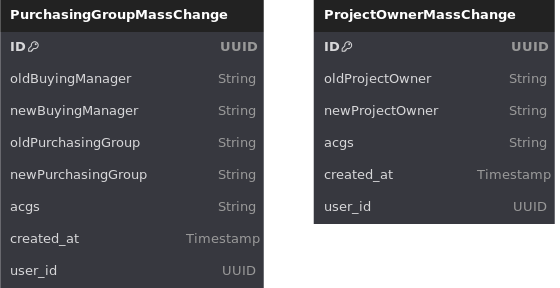
\includegraphics[width=.6\linewidth]{Images/MassChangeTables.png}
    \caption[Datenbanktabellen für Massenänderungen]{Datenbanktabellen für Massenänderungen}
    \label{fig:masschangetables}
\end{figure}

Wenn aus dem Frontend ein neuer Eintrag in einer der Entitäten erstellt wird, soll mit einer sogenannten \textit{Hook} in \gls{cap} das Ändern der Daten geschehen.
Diese \textit{Hooks} fangen das Erstellen der Enität ab und führen dann individuellen Code aus, in dem die gesendeten Daten verarbeitet werden können.

Bevor jedoch die Daten verarbeitet werden, muss überprüft werden, ob der Benutzer, der die Daten gesendet hat, die Berechtigung hat, diese Änderungen durchzuführen.
Falls dies nicht der Fall ist, soll ein Error an das Frontend gesendet und eine entsprechende Fehlernachricht angezeigt werden.
Besitzt der Benutzer jedoch die benötigte Berechtigung, sollen die Daten verarbeitet und validiert werden und die Änderungen in der Datenbank vorgenommen werden.

\subsection[Schrittweise Beschreibung der Implementierung]{Schrittweise Beschreibung der Implementierung}

In diesem Abschnitt werden die Implementierungsdetails aus dem vorherigen Abschnitt anhand von Codebeispielen schrittweise erläutert und erklärt.

\subsubsection{Frontend}
Die Implementierung des Frontends teilt sich in zwei Abschnitte auf. 
Zum einen die Erstellung der Views, welche die Darstellung der Seiten sein werden, und zum anderen die Erstellung der Controller, die Views mit Funktionalität zu versehen. 

\textbf{Erstellung der XML-Views:}

Für die Darstellung wurden, wie in Abbildung \ref{fig:appstructure} bereits dargestellt wurde, vier verschiendene \gls{xml}-Views angelegt.
Die \textit{App.view.xml}, \textit{BuyingManagerPurchasingGroup.view.xml}, \textit{ProjectOwner.view.xml} und die \textit{DeleteBuyingProjects.view.xml}.

Für die App-View wurden drei Hauptkomponenten benötigt.
Die Kopfzeile mit dem Titel der Seite, die Navigationsleiste zur Navigation zwischen den Unterseiten und den Unterseiten an sich, welche dynamisch mithilfe der Navigationsleiste angezeigt werden.
All diese Komponenten wurden innerhalb einer \textit{DynamicPage-Komponente} definiert, welche bereits Funktionalitäten für eine einfahrbare Kopfzeile und Navigationsleiste bietet.
So konnte die Kopfzeile als eine \textit{DynamicPageTitle und DynamicPageHeader-Komponente} als Titel und Header der DynamicPage hinzugefügt werden.
Wie das dann im Code für das Admin-UI aussieht, zeigt das fogende Listing:

\begin{lstlisting}[caption={Kopfzeile des App-Views}, language={XML}]
<f:DynamicPage class="sapUiNoContentPadding">
    <f:title>
        <f:DynamicPageTitle>
            <f:heading>
                <Title text="{i18n>titHeader}" class="sapUiSmallMarginTop" />
            </f:heading>
        </f:DynamicPageTitle>
    </f:title>
    <f:header>
        <f:DynamicPageHeader>
            <VBox>
                <Label text="{i18n>lblVersion}" />
            </VBox>
        </f:DynamicPageHeader>
    </f:header>
    ...
</f:DynamicPage>
\end{lstlisting}

Das \textit{text}-Attribut liefert den Text, der in dem Titel und dem Header angezeigt wird.
Dieser kommt in unserem Fall aus dem \textit{i18n}-Model, welches Text in verschiedenen Sprachen bereitstellt.
Das \textit{class}-Attribut ist für das Styling der Elemente verantwortlich. 
Hier wird eine von \gls{sapui5} vorgefertigte Klasse angegeben, um ein einheitliches Aussehen auf der ganzen Seite zu garantieren.

Für die Navigationsleiste und die Unterseiten wurden zwei \textit{Panel-Komponenten} verwendet, diese dienen als Container für den Inhalt der Komponenten und haben die Möglichkeit, sich ein- und ausklappen zu lassen.
Die Navigationsleiste wurde als eine Liste von \textit{ActionListItems} definiert, welche eine Art Knöpfe sind, die durch Attribute als ausgewählt angezeigt werden können.
Diese \textit{ActionListItems} werden anhand von vordefinierten Routen dynamisch generiert und sind somit jeweils an eine Route, beziehungsweise an eine Unterseite gebunden.
Durch Anklicken eines der \textit{ActionListItems} wird über den \gls{sapui5}-Router das richtige XML-View in den \textit{Panel-Container} für die Unterseiten geladen.

In dem folgenden Listing wird der Code für die beiden \textit{Panel-Komponenten} dargestellt, es wurden jedoch Attribute und Elemente, welche lediglich für das Aussehen der Komponenten zuständig sind, ausgelassen. 

\begin{lstlisting}[caption={Navigationsleisten- und Unterseiten-Container des Admin-UIs}, language={XML}]
...
<Panel>
    <List items="{routes>/routes}">
        <ActionListItem
            text="{
                parts: [
                    'routes>name'
                ], formatter: '.formatter.formatNavItemText'
            }"
            type="Navigation"
            navigated="{= ${routes>name} === ${routes>/currentRoute}}"
            press="onNavItemPress" />
    </List>
</Panel>
<Panel>
    <NavContainer id="navContainer" width="100%" height="100%" />
</Panel>
...
\end{lstlisting}

Die drei \gls{xml}-Views für die Unterseiten sind alle gleich aufgebaut und verwenden alle dieselben Komponenten zur Darstellung der \textit{Toolbar} zum Speichern der Änderungen und den Eingabefeldern.

Für die Toolbar wird die \textit{Toolbar-Komponente} von \gls{sapui5} verwendet und beinhaltet zwei Knöpfe.
Ein Knopf zum Speichern und ein Knopf, um alle Eingabefelder zu leeren. 
Im folgenden Listing wird der Code für die Toolbar, welche auf allen Seiten weitestgehend identisch ist, dargestellt:

\begin{lstlisting}[caption={Toolbar der Unterseiten}, label={lst:toolbar}, language={XML}]
<Toolbar id="toolbar" design="Solid">
    <ToolbarSpacer />
    <Button text="{i18n>btnSaveChanges}" type="Emphasized" press="onSaveChangesPress" />
    <Button text="{i18n>btnClear}" press="onClearPress" />
</Toolbar>
\end{lstlisting}

Die Eingabefelder wurden mit \textit{Input-Komponenten} umgesetzt, da diese bereits Funktionalitäten für intelligente Vorschläge, wie in Anforderung \ref{Tab:A3} beschrieben, besitzen.
Für eine bessere Formatierung wurde jedes Eingabefeld und dessen Titel, welcher als \textit{Label-Komponente} dargestellt wird, in einer \textit{VBox-Komponente} platziert.
In dem folgenden Listing wird der Code für das Eingabefeld beispielhaft an einem Eingabefeld auf der ProjectOwner.view.xml Unterseite dargestellt:

\begin{lstlisting}[caption={Eingabefeld für Unterseiten}, language={XML}]
<VBox width="100%">
    <Label text="{i18n>lblOldBuyingManager}" required="true" />
    <Input
        id="oldBuyingManagerInput"
        value="{form>/oldBuyingManager}"
        placeholder="{i18n>txtEmailPlaceholder1}"
        required="true"
        suggestionItems="{/AppUsers}"
        showSuggestion="true"
        suggest="onSuggest($event, 'user')"
        suggestionItemSelected="onSuggestionItemSelected">
        <core:Item key="{id}" text="{id}" />
    </Input>
</VBox>
\end{lstlisting}

Die Attribute \textit{suggest} und \textit{suggestionItemSelected} der Input-Komponente bekommen die Namen von Funktionen übergeben, welche in einem Controller für die Views definiert sind.
Die Funktion dieser Funktionen ist es, die intelligenten Vorschläge anhand der Benutzereingabe anzuzeigen und beim Auswählen eines der Vorschläge diesen Wert für das Feld zu übernehmen.
Das Attribut \textit{required} ist dafür da anzuzeigen, ob das Eingabefeld ein Pflichtfeld ist.
Wird dieses auf \textit{true} gesetzt, wird vor dem Speichern überprüft, ob in diesem Feld etwas eingegeben wurde.

\textbf{Erstellung der Controller:}

Einige Funktionalitäten sind in allen Unterseiten identisch, daher wurde für diese Funktionen ein BaseController erstellt.
Funktionen in diesem Controller stehen allen Views zur Verfügung, wodurch der Code für diese Funktionalitäten nur einmal geschrieben werden musste.

Andere Funktionalitäten sind jedoch spezifisch für eine Unterseite oder mussten unterschiedlich implementiert werden, da es zum Beispiel unterschiedliche Eingabefelder auf den Seiten gibt.
Eine dieser Funktionen ist die \textit{onSaveChangesPress}-Funktion aus Listing \ref{lst:toolbar}, die für das Speichern der Eingabefelder zuständig ist.

\begin{lstlisting}[caption={onSaveChangesPress Funktion}]
onSaveChangesPress(event: Button$PressEvent): void {
    const formModel = this.getModel<JSONModel>("form"),
            isFormValid = this.validateInputFields(this.allInputIDs);

    if (!isFormValid) {
        event.getSource().setEnabled(false);
        return;
    }

    if (!formModel) return;

    const {
        oldProjectOwner,
        newProjectOwner,
        SCGs
    } = formModel.getData();

    this.createSaveChangesMessageBox(
        "/ProjectOwnerMassChange", 
        {                
            oldProjectOwner,
            newProjectOwner,
            acgs: SCGs
        },
        this.allInputIDs
    );
}
\end{lstlisting}

In dieser Funktion werden die Eingabefelder validiert, indem überprüft wird, ob alle Pflichtfelder ausgefüllt sind.
Wenn dies der Fall ist, wird mit den Werten der Eingabefelder ein neuer Eintrag in der passenden Entität im Backend erstellt.
Der Tabellenname ist für die verschiedenen Unterseiten unterschiedlich und daher wird dieser zusammen mit den Daten an die \textit{createSaveChangesMessageBox}-Funktion im BaseController gesendet.
Diese Funktion ist im folgenden Listing zu sehen:

\begin{lstlisting}[caption={createSaveChangesMessageBox Funktion}]
protected createSaveChangesMessageBox(sPath: string, formData: object, inputIDs: string[]): void {
    const resourceBundle = this.getI18nResourceBundle();
    if (!resourceBundle) {
        return;
    }
    const saveAction = resourceBundle.getText("btnSave") || "Save";
    MessageBox.confirm(
        resourceBundle.getText("txtConfirmDialog") || "",
        {
            title: resourceBundle.getText("titConfirmDialog") || "",
            actions: [saveAction, MessageBox.Action.CANCEL],
            emphasizedAction: saveAction,
            onClose: (action: string) => {
                if (action === saveAction) {
                    this.submitChanges(sPath, formData, inputIDs);
                }
            }
        }
    );
} 
\end{lstlisting}

Dies ist eine Funktion im BaseController, welche eine \textit{MessageBox-Komponente} erstellt, um den Nutzer um eine weitere Bestätigung zu bitten.
Bestätigt der Benutzer seine Entscheidung, wird die \textit{submitChanges}-Funktion aufgerufen.

\begin{lstlisting}[caption={submitChanges Funktion}]
protected submitChanges(sPath: string, oData: object, inputIDs: string[]): void {
    const   viewModel = this.getModel<JSONModel>("objectView"),
            model = this.getModel<ODataModel>();

    if (!model || !viewModel) return;

    viewModel.setProperty("/busy", true);
    model.create(sPath, oData,
        {
            success: () => {
                this.clearAllFields(inputIDs);
                this.onSubmitSuccess();
            },
            error: this.onSubmitError.bind(this),
        }
    );
} 
\end{lstlisting}

Diese Funktion ist dafür verantwortlich, die übergebenen Daten an das Backend zu senden.
Um das zu tun, wird in dem \gls{odata}-Model, welches mit dem Backend verbunden ist, ein neuer Eintrag erstellt.
Dafür benötigt es die Namen der Entität, sowie die Daten, die in die Entität geschrieben werden sollen.
Ist das Erstellen des neuen Eintrages erfolgreich, werden alle Eingabefelder geleert und es wird eine Meldung angezeigt, dass das Speichern erfolgreich war.
Im Fall, dass das Erstellen nicht erfolgreich war, wird eine Fehlernachricht angezeigt.

\subsubsection[Backend]{Backend}

Nachdem die Daten von dem Frontend an das Backend gesendet wurden, müssen diese dort noch verarbeitet werden und die von den Änderungen betroffenen Entitäten müssen bearbeitet werden.
Die Beschreibung dieser Funktionalität wird im Folgenden schrittweise beschrieben.

Sobald im Frontend eine Anfrage an das Backend gesendet wird, um einen neuen Eintrag in der Entität zu erstellen, wird diese Anfrage von SAP CAP abgefangen.
Dies geschieht in der \textit{srv.on} Funktion, welche bestimmte Events abfangen kann.
Sie hat drei Parameter, das Event, welches abgefangen werden soll, den Namen der Entität und eine Handlerfunktion, die aufgeführt wird, wenn eine Anfrage abgefangen wurde.

In diesem Fall ist das Event das \textit{CREATE} Event, welches beim Erstellen eines neuen Eintrags aufgerufen wird.
Der Name der Entität ist abhängig von der Unterseite, von der die Anfrage gestellt wurde.
Die Handlerfunktion hat zwei Parameter, die Anfrage, in der die Daten die gesendet wurden sowie weitere Informationen über die Anfrage, wie den Benutzer, der die Anfrage gestellt hat, stehen.

Im Folgenden wird das Codebeispiel nur für eine der Funktionalitäten dargestellt, da der einzige Unterschied die aufgerufene Funktion ist.
\begin{lstlisting}[caption={srv.on Funktion zum Abfangen der Anfrage}]    
srv.on('CREATE', 'PurchasingGroupMassChange', async (req, next) => {
    const whitelistedMassChangeUsers = process.env.ADMIN_UI_USERS ? process.env.ADMIN_UI_USERS.split(',') : []
    if(whitelistedMassChangeUsers.indexOf(req.user.id.toLowerCase()) < 0) {
        req.error(400, 'Invalid user')
    } else {
        try {
            await projectService.purchasingGroupMassChange(req)
            return await next()
        } catch (e) {
            logAndThrowError(log, 'performing purchasing group mass change', e, req.data)
        }
    }
})
\end{lstlisting}

In unserer Handlerfunktion ist das Erste, was geprüft wird, ob der Benutzer, der die Anfrage gestellt hat, die passenden Rechte für eine solche Anfrage besitzt.
Ist dies nicht der Fall, wird eine Fehlernachricht zurückgesendet.
Besitzt der Benutzer die passenden Rechte, wird eine Funktion aufgerufen, welche die Validierung und Verarbeitung der Daten übernimmt.

Hierbei wurde jedoch zwischen der Funktionalität, Kaufprojekte zu löschen und Kaufprojekte zu bearbeiten, unterschieden.
Die Funktion, Kaufprojekte zu löschen, benötigte keine weitere Verarbeitung der Daten.
Um ein Kaufprojekt zu löschen, beziehungsweise ein Kaufprojekt als gelöscht zu markieren, musste lediglich das Attribut \textit{deleted} auf \textit{true} gesetzt werden und der Eintrag in der \textit{BuyingProjectTableView} Entität gelöscht werden.

Für die Funktionalitäten des Aktualisierens der Projektmanager und der Käufergruppe sowie des Projektowners, müssen die Daten noch validiert und verarbeitet werden. 
Dafür wird zuerst überprüft, ob alle benötigten Daten angekommen sind und ob diese das korrekte Format besitzen.
Falls dies nicht der Fall ist, wird eine Fehlernachricht zurückgesendet.
Nachdem die Validierung abgeschlossen ist und es zu keinem Fehler gekommen ist, werden die betroffenen Entitäten aktualisiert. 

Die verschiedenen Unterseiten erfordern eine unterschiedliche Art und Weise, wie die Daten aktualisiert werden, daher wurden in diesem Schritt verschiedene Funktionen aufgerufen.
Für die Aktualisierung der Projektmanager und Käufergruppen wird zuerst die neue Käufergruppe hinzugefügt und dem neuen Projektmanager zugewiesen.

\begin{lstlisting}[caption={Einfügen und Aktualisieren der Käufergruppe}]
async function insertNewPurchGroup(db, newPurchGroup) {
    const { PurchasingGroup } = db.entities('com.company.buyingcockpit.buyingProject')
    await db.run(INSERT.into(PurchasingGroup)
                        .entries({ ID: newPurchGroup, Name: newPurchGroup }))
}

async function updatePurchGroupOfNewManager(db, newPurchGroup, newBuyingManager) {
    const { AppUser } = db.entities('com.company.buyingcockpit.common')
    await db.run(UPDATE(AppUser)
        .with({ purchaseGroup: newPurchGroup })
        .where({ ID: newBuyingManager }))
}
\end{lstlisting}

Die \textit{db.run}-Funktion ist eine Funktion von \gls{cap} die verschiedene Datenbankoperationen durchführen kann.
In den beiden Funktionen wird \textit{INSERT} zum Hinzufügen der neuen Käufergruppe verwendet und \textit{UPDATE}, um den Projektmanager zu aktualisieren.

Nachdem die Käufergruppe aktualisiert wurde, müssen die Projektländer aktualisiert werden.
Die Projektländer mussten hierfür nach zwei Kriterien gefiltert werden.
Zum einen danach, dass der alte Projektmanager als Projektmanager in dem Projektland eingetragen ist, sowie, dass das Kaufprojekt, zu dem das Projektland gehört, die \gls{scg} besitzt, die der Benutzer gegebenenfalls angegeben hat.

Das Filtern nach dem aktuellen Projektmanager konnte mit einer \textit{where}-Bedingung der \textit{SELECT}-Operation geschehen:

\begin{lstlisting}[caption={SELECT-Operation für Projektländer}]
const projectCountriesToUpdate = await db.run(
    SELECT.from(ProjectCountry)
        .columns('ID', 'project_ID')
        .where({ buyingManager_ID: oldBuyingManager, or: { purchasingGroup_ID: oldPurchGroup } })
)
\end{lstlisting}

Um diese Projektländer dann nach den \glspl{scg} zu filtern, wurde mehr Berechnungsaufwand benötigt, da diese nicht in den Projektländern gespeichert sind, sondern in dem dazugehörigen Kaufprojekt.
Daher wurde eine weitere Funktion geschrieben, welche die vor gefilterten Projektländer nach den \glspl{scg} filtert:

\begin{lstlisting}[caption={\gls{scg} Filterfunktion für Projektländer}]
async function filterProjectCountriesBySCGs(db, projectCountries, scgs) {
    const { BuyingProject } = db.entities('com.company.buyingcockpit.buyingProject')
    const projectIds = [...new Set(projectCountries.map((pc) => pc.project_ID))]

    if (scgs.length > 0 && projectIds.length > 0) {
        const projects = await db.run(
            SELECT.from(BuyingProject)
                .columns((project) => {
                    project('ID')
                    project.commodity((commodity) => {
                        commodity('Code')
                    })
                })
                .where({ ID: { in: projectIds } })
        )

        const projectsMap = {}
        for (const project of projects) {
            projectsMap[project.ID] = project
        }

        return projectCountries.filter((pc) => {
            const project = projectsMap[pc.project_ID]
            return !!project && !!project.commodity && scgs.indexOf(project.commodity.Code) >= 0
        })
    } else {
        return projectCountries
    }
}
\end{lstlisting}

In dieser Funktion werden zuerst alle Kaufprojekte (BuyingProject) mit der \textit{SELECT}-Operation gesucht, welche in den Projektländern als Kaufprojekt angegeben sind.
Anhand dieser Kaufprojekte werden dann die Projektländer (ProjectCountries) gefiltert.
Dafür wird überprüft, ob der \textit{Commodity Code} (auch \gls{scg}) des zu dem Projektland gehörenden Kaufprojektes in der Liste der angegebenen \glspl{scg} ist.
Diese gefilterte Liste wird dann zurückgegeben.
Anhand dieser Liste konnten dann die betroffenen Entitäten aktualisiert werden.

Sind diese Entitäten aktualisiert, ist die Verarbeitung der Daten vollendet.
Das Letzte was nun noch geschieht, ist, dass ein Eintrag mit den Änderungen, die vorgenommen wurden, erstellt wird, um diese zu einem späteren Zeitpunkt nachvollziehen zu können und gegebenenfalls rückgängig zu machen.


\subsection[Herausforderungen und Problemlösungen]{Herausforderungen und Problemlösungen}

Ein zentrales Problem war die Handhabung der unterschiedlichen Anforderungen in den Controllern.
Während einige Funktionalitäten spezifisch für eine Unterseite waren, mussten andere auf mehreren Seiten gleich funktionieren.
Um das DRY-Prinzip (Don't Repeat Yourself) zu beachten, war es wichtig, den Code, der von mehreren Seiten genutzt wird, zu abstrahieren.

Um dieses Problem zu lösen, wurden die gemeinsamen Logiken der Controller in den BaseController ausgelagert.
Dadurch konnte sichergestellt werden, dass wiederkehrende Logik nicht mehrfach in den einzelnen Controllern dupliziert wird.
Anstatt den Code für API-Aufrufe oder Datenvalidierung in jedem Controller zu wiederholen, wurden diese Funktionen in den BaseController integriert.
Die spezifischen Controller konnten dann von dieser Klasse erben und nur die für die Unterseiten benötigten Funktionen implementieren.
So blieb der Code flexibel und konnte den spezifischen Anforderungen der Unterseiten gerecht werden, ohne redundanten Code schreiben zu müssen.

Zusätzlich wurden Hilfsfunktionen erstellt, die häufig genutzte Logik wie die Validierung von Benutzereingaben oder die Verarbeitung von Daten zentralisiert.
Diese Hilfsfunktionen konnten dann von allen Controllern aufgerufen werden, was den Code nicht nur wiederverwendbar, sondern auch wartbarer machte.

Durch diese Maßnahmen konnten die unterschiedlichen Anforderungen der Unterseiten effizient gemanaget und gleichzeitig sichergestellt werden, dass das DRY-Prinzip beachtet wird.